% Options for packages loaded elsewhere
\PassOptionsToPackage{unicode}{hyperref}
\PassOptionsToPackage{hyphens}{url}
%
\documentclass[
]{article}
\usepackage{amsmath,amssymb}
\usepackage{lmodern}
\usepackage{iftex}
\ifPDFTeX
  \usepackage[T1]{fontenc}
  \usepackage[utf8]{inputenc}
  \usepackage{textcomp} % provide euro and other symbols
\else % if luatex or xetex
  \usepackage{unicode-math}
  \defaultfontfeatures{Scale=MatchLowercase}
  \defaultfontfeatures[\rmfamily]{Ligatures=TeX,Scale=1}
\fi
% Use upquote if available, for straight quotes in verbatim environments
\IfFileExists{upquote.sty}{\usepackage{upquote}}{}
\IfFileExists{microtype.sty}{% use microtype if available
  \usepackage[]{microtype}
  \UseMicrotypeSet[protrusion]{basicmath} % disable protrusion for tt fonts
}{}
\makeatletter
\@ifundefined{KOMAClassName}{% if non-KOMA class
  \IfFileExists{parskip.sty}{%
    \usepackage{parskip}
  }{% else
    \setlength{\parindent}{0pt}
    \setlength{\parskip}{6pt plus 2pt minus 1pt}}
}{% if KOMA class
  \KOMAoptions{parskip=half}}
\makeatother
\usepackage{xcolor}
\usepackage[margin=1in]{geometry}
\usepackage{color}
\usepackage{fancyvrb}
\newcommand{\VerbBar}{|}
\newcommand{\VERB}{\Verb[commandchars=\\\{\}]}
\DefineVerbatimEnvironment{Highlighting}{Verbatim}{commandchars=\\\{\}}
% Add ',fontsize=\small' for more characters per line
\usepackage{framed}
\definecolor{shadecolor}{RGB}{248,248,248}
\newenvironment{Shaded}{\begin{snugshade}}{\end{snugshade}}
\newcommand{\AlertTok}[1]{\textcolor[rgb]{0.94,0.16,0.16}{#1}}
\newcommand{\AnnotationTok}[1]{\textcolor[rgb]{0.56,0.35,0.01}{\textbf{\textit{#1}}}}
\newcommand{\AttributeTok}[1]{\textcolor[rgb]{0.77,0.63,0.00}{#1}}
\newcommand{\BaseNTok}[1]{\textcolor[rgb]{0.00,0.00,0.81}{#1}}
\newcommand{\BuiltInTok}[1]{#1}
\newcommand{\CharTok}[1]{\textcolor[rgb]{0.31,0.60,0.02}{#1}}
\newcommand{\CommentTok}[1]{\textcolor[rgb]{0.56,0.35,0.01}{\textit{#1}}}
\newcommand{\CommentVarTok}[1]{\textcolor[rgb]{0.56,0.35,0.01}{\textbf{\textit{#1}}}}
\newcommand{\ConstantTok}[1]{\textcolor[rgb]{0.00,0.00,0.00}{#1}}
\newcommand{\ControlFlowTok}[1]{\textcolor[rgb]{0.13,0.29,0.53}{\textbf{#1}}}
\newcommand{\DataTypeTok}[1]{\textcolor[rgb]{0.13,0.29,0.53}{#1}}
\newcommand{\DecValTok}[1]{\textcolor[rgb]{0.00,0.00,0.81}{#1}}
\newcommand{\DocumentationTok}[1]{\textcolor[rgb]{0.56,0.35,0.01}{\textbf{\textit{#1}}}}
\newcommand{\ErrorTok}[1]{\textcolor[rgb]{0.64,0.00,0.00}{\textbf{#1}}}
\newcommand{\ExtensionTok}[1]{#1}
\newcommand{\FloatTok}[1]{\textcolor[rgb]{0.00,0.00,0.81}{#1}}
\newcommand{\FunctionTok}[1]{\textcolor[rgb]{0.00,0.00,0.00}{#1}}
\newcommand{\ImportTok}[1]{#1}
\newcommand{\InformationTok}[1]{\textcolor[rgb]{0.56,0.35,0.01}{\textbf{\textit{#1}}}}
\newcommand{\KeywordTok}[1]{\textcolor[rgb]{0.13,0.29,0.53}{\textbf{#1}}}
\newcommand{\NormalTok}[1]{#1}
\newcommand{\OperatorTok}[1]{\textcolor[rgb]{0.81,0.36,0.00}{\textbf{#1}}}
\newcommand{\OtherTok}[1]{\textcolor[rgb]{0.56,0.35,0.01}{#1}}
\newcommand{\PreprocessorTok}[1]{\textcolor[rgb]{0.56,0.35,0.01}{\textit{#1}}}
\newcommand{\RegionMarkerTok}[1]{#1}
\newcommand{\SpecialCharTok}[1]{\textcolor[rgb]{0.00,0.00,0.00}{#1}}
\newcommand{\SpecialStringTok}[1]{\textcolor[rgb]{0.31,0.60,0.02}{#1}}
\newcommand{\StringTok}[1]{\textcolor[rgb]{0.31,0.60,0.02}{#1}}
\newcommand{\VariableTok}[1]{\textcolor[rgb]{0.00,0.00,0.00}{#1}}
\newcommand{\VerbatimStringTok}[1]{\textcolor[rgb]{0.31,0.60,0.02}{#1}}
\newcommand{\WarningTok}[1]{\textcolor[rgb]{0.56,0.35,0.01}{\textbf{\textit{#1}}}}
\usepackage{graphicx}
\makeatletter
\def\maxwidth{\ifdim\Gin@nat@width>\linewidth\linewidth\else\Gin@nat@width\fi}
\def\maxheight{\ifdim\Gin@nat@height>\textheight\textheight\else\Gin@nat@height\fi}
\makeatother
% Scale images if necessary, so that they will not overflow the page
% margins by default, and it is still possible to overwrite the defaults
% using explicit options in \includegraphics[width, height, ...]{}
\setkeys{Gin}{width=\maxwidth,height=\maxheight,keepaspectratio}
% Set default figure placement to htbp
\makeatletter
\def\fps@figure{htbp}
\makeatother
\setlength{\emergencystretch}{3em} % prevent overfull lines
\providecommand{\tightlist}{%
  \setlength{\itemsep}{0pt}\setlength{\parskip}{0pt}}
\setcounter{secnumdepth}{-\maxdimen} % remove section numbering
\ifLuaTeX
  \usepackage{selnolig}  % disable illegal ligatures
\fi
\IfFileExists{bookmark.sty}{\usepackage{bookmark}}{\usepackage{hyperref}}
\IfFileExists{xurl.sty}{\usepackage{xurl}}{} % add URL line breaks if available
\urlstyle{same} % disable monospaced font for URLs
\hypersetup{
  pdftitle={HUDM6026 Homework\_05},
  pdfauthor={Chenguang Pan \& Seng Lei},
  hidelinks,
  pdfcreator={LaTeX via pandoc}}

\title{HUDM6026 Homework\_05}
\author{Chenguang Pan \& Seng Lei}
\date{Feb 24, 2023}

\begin{document}
\maketitle

\hypertarget{q1}{%
\subsection{Q1:}\label{q1}}

\emph{Determine the first derivative of f and encode it in a function
called f\_prime.}

\textbf{MY SOLUTION:}\\
Based on chain rule, the first derivative of \(f(x)\) is
\[f(x)' = \frac{-2x}{x^2+1}+\frac{1}{3}x^{-\frac{2}{3}}\]. Based on this
equation, I write the code below. Certainly, we can use the R-built-in
function to get the derivative quickly.

\begin{Shaded}
\begin{Highlighting}[]
\SpecialCharTok{\textgreater{}}\NormalTok{ f\_prime }\OtherTok{\textless{}{-}} \ControlFlowTok{function}\NormalTok{(x) \{}
\SpecialCharTok{+}\NormalTok{   out\_ }\OtherTok{\textless{}{-}}\NormalTok{ (}\SpecialCharTok{{-}}\DecValTok{2}\SpecialCharTok{*}\NormalTok{x)}\SpecialCharTok{/}\NormalTok{(x}\SpecialCharTok{\^{}}\DecValTok{2} \SpecialCharTok{+} \DecValTok{1}\NormalTok{) }\SpecialCharTok{+}\NormalTok{ (}\DecValTok{1}\SpecialCharTok{/}\DecValTok{3}\NormalTok{)}\SpecialCharTok{*}\NormalTok{(x}\SpecialCharTok{\^{}}\NormalTok{(}\SpecialCharTok{{-}}\DecValTok{2}\SpecialCharTok{/}\DecValTok{3}\NormalTok{))}
\SpecialCharTok{+}   \FunctionTok{return}\NormalTok{(out\_)}
\SpecialCharTok{+}\NormalTok{ \}}
\SpecialCharTok{\textgreater{}} \CommentTok{\# since this question requires the maximum, I use {-}1 times the function.}
\ErrorTok{\textgreater{}}\NormalTok{ f\_prime\_neg }\OtherTok{\textless{}{-}} \ControlFlowTok{function}\NormalTok{(x)\{}
\SpecialCharTok{+}\NormalTok{   out\_ }\OtherTok{\textless{}{-}}\NormalTok{ (}\SpecialCharTok{{-}}\DecValTok{2}\SpecialCharTok{*}\NormalTok{x)}\SpecialCharTok{/}\NormalTok{(x}\SpecialCharTok{\^{}}\DecValTok{2} \SpecialCharTok{+} \DecValTok{1}\NormalTok{) }\SpecialCharTok{+}\NormalTok{ (}\DecValTok{1}\SpecialCharTok{/}\DecValTok{3}\NormalTok{)}\SpecialCharTok{*}\NormalTok{(x}\SpecialCharTok{\^{}}\NormalTok{(}\SpecialCharTok{{-}}\DecValTok{2}\SpecialCharTok{/}\DecValTok{3}\NormalTok{))}
\SpecialCharTok{+}\NormalTok{   out\_ }\OtherTok{\textless{}{-}}\NormalTok{ out\_}\SpecialCharTok{*}\NormalTok{(}\SpecialCharTok{{-}}\DecValTok{1}\NormalTok{)}
\SpecialCharTok{+}   \FunctionTok{return}\NormalTok{(out\_)}
\SpecialCharTok{+}\NormalTok{ \}}
\end{Highlighting}
\end{Shaded}

\hypertarget{q2}{%
\subsection{Q2:}\label{q2}}

\emph{Create a plot of f and f on {[}0,4{]} in different colors and line
types and add a legend.} \textbf{MY SOLUTION:}

\begin{Shaded}
\begin{Highlighting}[]
\SpecialCharTok{\textgreater{}} \CommentTok{\# write the original function with the name of f\_}
\ErrorTok{\textgreater{}}\NormalTok{ f\_ }\OtherTok{\textless{}{-}} \ControlFlowTok{function}\NormalTok{(x)\{}
\SpecialCharTok{+}\NormalTok{   out\_ }\OtherTok{\textless{}{-}}\NormalTok{ (}\SpecialCharTok{{-}}\DecValTok{1}\NormalTok{)}\SpecialCharTok{*}\FunctionTok{log}\NormalTok{(x}\SpecialCharTok{\^{}}\DecValTok{2} \SpecialCharTok{+} \DecValTok{1}\NormalTok{) }\SpecialCharTok{+}\NormalTok{ x}\SpecialCharTok{\^{}}\NormalTok{(}\DecValTok{1}\SpecialCharTok{/}\DecValTok{3}\NormalTok{)}
\SpecialCharTok{+}   \FunctionTok{return}\NormalTok{(out\_)\}}
\SpecialCharTok{\textgreater{}} \CommentTok{\# since this question requires the maximum, I use {-}1 times the function.}
\ErrorTok{\textgreater{}}\NormalTok{ f\_neg }\OtherTok{\textless{}{-}} \ControlFlowTok{function}\NormalTok{(x)\{}
\SpecialCharTok{+}\NormalTok{   out\_ }\OtherTok{\textless{}{-}}\NormalTok{ (}\SpecialCharTok{{-}}\DecValTok{1}\NormalTok{)}\SpecialCharTok{*}\FunctionTok{log}\NormalTok{(x}\SpecialCharTok{\^{}}\DecValTok{2} \SpecialCharTok{+} \DecValTok{1}\NormalTok{) }\SpecialCharTok{+}\NormalTok{ x}\SpecialCharTok{\^{}}\NormalTok{(}\DecValTok{1}\SpecialCharTok{/}\DecValTok{3}\NormalTok{)}
\SpecialCharTok{+}   \FunctionTok{return}\NormalTok{(out\_}\SpecialCharTok{*}\NormalTok{(}\SpecialCharTok{{-}}\DecValTok{1}\NormalTok{))\}}
\SpecialCharTok{\textgreater{}} 
\ErrorTok{\textgreater{}} \CommentTok{\# first plot the original function}
\ErrorTok{\textgreater{}}\NormalTok{ x }\OtherTok{\textless{}{-}} \FunctionTok{seq}\NormalTok{(}\DecValTok{0}\NormalTok{,}\DecValTok{4}\NormalTok{,}\FloatTok{0.01}\NormalTok{)}
\SpecialCharTok{\textgreater{}} \CommentTok{\# plot the original function with blue line}
\ErrorTok{\textgreater{}} \FunctionTok{plot}\NormalTok{(x, }\FunctionTok{f\_}\NormalTok{(x), }\AttributeTok{col=}\StringTok{"blue"}\NormalTok{, }\AttributeTok{type =} \StringTok{"l"}\NormalTok{, }\AttributeTok{ylim =} \FunctionTok{c}\NormalTok{(}\SpecialCharTok{{-}}\FloatTok{1.5}\NormalTok{,}\DecValTok{1}\NormalTok{))}
\SpecialCharTok{\textgreater{}} \CommentTok{\# plot the first derivative with red line}
\ErrorTok{\textgreater{}} \FunctionTok{lines}\NormalTok{(x, }\FunctionTok{f\_prime}\NormalTok{(x), }\AttributeTok{col=}\StringTok{"red"}\NormalTok{, }\AttributeTok{type =} \StringTok{"l"}\NormalTok{)}
\SpecialCharTok{\textgreater{}} \CommentTok{\# add the legend}
\ErrorTok{\textgreater{}} \FunctionTok{legend}\NormalTok{(}\DecValTok{3}\NormalTok{,}\DecValTok{1}\NormalTok{, }\AttributeTok{inset =} \FloatTok{0.1}\NormalTok{, }\FunctionTok{c}\NormalTok{(}\StringTok{"f\_"}\NormalTok{,}\StringTok{"f\_prime"}\NormalTok{), }\AttributeTok{lty =} \DecValTok{1}\NormalTok{, }
\SpecialCharTok{+}        \AttributeTok{col =} \FunctionTok{c}\NormalTok{(}\StringTok{"blue"}\NormalTok{,}\StringTok{"red"}\NormalTok{), }\AttributeTok{title=}\StringTok{"line Type"}\NormalTok{)}
\SpecialCharTok{\textgreater{}} \CommentTok{\# add a horizontal line to indicate the y=0}
\ErrorTok{\textgreater{}} \FunctionTok{abline}\NormalTok{(}\AttributeTok{h=}\DecValTok{0}\NormalTok{,}\AttributeTok{lty=}\DecValTok{3}\NormalTok{)}
\SpecialCharTok{\textgreater{}} \FunctionTok{abline}\NormalTok{(}\AttributeTok{v=}\FloatTok{0.3683525}\NormalTok{,}\AttributeTok{lty=}\DecValTok{3}\NormalTok{)}
\SpecialCharTok{\textgreater{}} \FunctionTok{mtext}\NormalTok{(}\StringTok{"Figure 1. The Lines of the Given Function and it\textquotesingle{}s First Derivative"}\NormalTok{,}
\SpecialCharTok{+}       \AttributeTok{side =} \DecValTok{3}\NormalTok{,}
\SpecialCharTok{+}       \AttributeTok{line =} \SpecialCharTok{{-}}\DecValTok{2}\NormalTok{,}
\SpecialCharTok{+}       \AttributeTok{outer =}\NormalTok{ T)}
\end{Highlighting}
\end{Shaded}

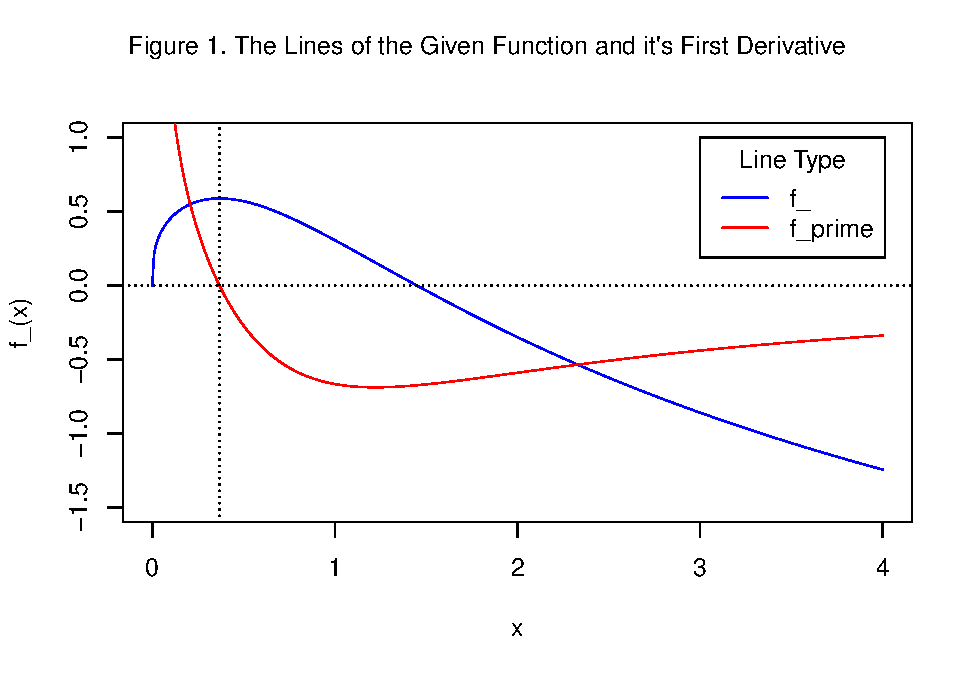
\includegraphics{Homework_05_Pan-Lei_files/figure-latex/unnamed-chunk-2-1.pdf}

\hypertarget{q3}{%
\subsection{Q3:}\label{q3}}

\emph{Finish the functions that I started in the R code notes for
univariate optimization for the golden section search, the bisection
method, and Newton's method.}

\textbf{MY SOLUTION:}\\
\#\#\# 3.1 The Golden Section Search

\begin{Shaded}
\begin{Highlighting}[]
\SpecialCharTok{\textgreater{}}\NormalTok{ golden }\OtherTok{\textless{}{-}} \ControlFlowTok{function}\NormalTok{(f, int, }\AttributeTok{precision =} \FloatTok{1e{-}6}\NormalTok{)}
\SpecialCharTok{+}\NormalTok{ \{}
\SpecialCharTok{+}\NormalTok{   rho }\OtherTok{\textless{}{-}}\NormalTok{ (}\DecValTok{3}\SpecialCharTok{{-}}\FunctionTok{sqrt}\NormalTok{(}\DecValTok{5}\NormalTok{))}\SpecialCharTok{/}\DecValTok{2} \CommentTok{\# ::: Golden ratio}
\SpecialCharTok{+}   \CommentTok{\# ::: Work out first iteration here}
\SpecialCharTok{+}\NormalTok{   f\_a }\OtherTok{\textless{}{-}} \FunctionTok{f}\NormalTok{(int[}\DecValTok{1}\NormalTok{] }\SpecialCharTok{+}\NormalTok{ rho}\SpecialCharTok{*}\NormalTok{(}\FunctionTok{diff}\NormalTok{(int)))}
\SpecialCharTok{+}\NormalTok{   f\_b }\OtherTok{\textless{}{-}} \FunctionTok{f}\NormalTok{(int[}\DecValTok{2}\NormalTok{] }\SpecialCharTok{{-}}\NormalTok{ rho}\SpecialCharTok{*}\NormalTok{(}\FunctionTok{diff}\NormalTok{(int)))}
\SpecialCharTok{+}   \DocumentationTok{\#\#\# How many iterations will we need to reach the desired precision?}
\SpecialCharTok{+}\NormalTok{   N }\OtherTok{\textless{}{-}} \FunctionTok{ceiling}\NormalTok{(}\FunctionTok{log}\NormalTok{(precision}\SpecialCharTok{/}\NormalTok{(}\FunctionTok{diff}\NormalTok{(int)))}\SpecialCharTok{/}\FunctionTok{log}\NormalTok{(}\DecValTok{1}\SpecialCharTok{{-}}\NormalTok{rho))}
\SpecialCharTok{+}   \ControlFlowTok{for}\NormalTok{ (i }\ControlFlowTok{in} \DecValTok{1}\SpecialCharTok{:}\NormalTok{(N))                    }\CommentTok{\# index the number of iterations}
\SpecialCharTok{+}\NormalTok{   \{}
\SpecialCharTok{+}     \ControlFlowTok{if}\NormalTok{ (f\_a }\SpecialCharTok{\textless{}}\NormalTok{ f\_b)  }
\SpecialCharTok{+}\NormalTok{     \{}
\SpecialCharTok{+}\NormalTok{       int[}\DecValTok{2}\NormalTok{] }\OtherTok{\textless{}{-}}\NormalTok{ int[}\DecValTok{2}\NormalTok{] }\SpecialCharTok{{-}}\NormalTok{ rho}\SpecialCharTok{*}\NormalTok{(}\FunctionTok{diff}\NormalTok{(int))}
\SpecialCharTok{+}\NormalTok{       f\_b }\OtherTok{\textless{}{-}} \FunctionTok{f}\NormalTok{(int[}\DecValTok{2}\NormalTok{])}
\SpecialCharTok{+}\NormalTok{     \} }\ControlFlowTok{else}\NormalTok{\{}
\SpecialCharTok{+}       \ControlFlowTok{if}\NormalTok{ (f\_a }\SpecialCharTok{\textgreater{}=}\NormalTok{ f\_b)}
\SpecialCharTok{+}\NormalTok{       \{}
\SpecialCharTok{+}\NormalTok{         int[}\DecValTok{1}\NormalTok{] }\OtherTok{\textless{}{-}}\NormalTok{ int[}\DecValTok{1}\NormalTok{] }\SpecialCharTok{+}\NormalTok{ rho}\SpecialCharTok{*}\NormalTok{(}\FunctionTok{diff}\NormalTok{(int))}
\SpecialCharTok{+}\NormalTok{         f\_a }\OtherTok{\textless{}{-}} \FunctionTok{f}\NormalTok{(int[}\DecValTok{1}\NormalTok{])}
\SpecialCharTok{+}\NormalTok{       \} \}}
\SpecialCharTok{+}\NormalTok{   \}}
\SpecialCharTok{+}\NormalTok{   int}
\SpecialCharTok{+}   \FunctionTok{print}\NormalTok{(}\FunctionTok{paste0}\NormalTok{(}\StringTok{"Iteration for "}\NormalTok{,N,}\StringTok{" times;"}\NormalTok{,}
\SpecialCharTok{+}                \StringTok{" The maximum value is at"}\NormalTok{, }\FunctionTok{round}\NormalTok{(int[}\DecValTok{1}\NormalTok{],}\DecValTok{6}\NormalTok{)))}
\SpecialCharTok{+}\NormalTok{ \}}
\end{Highlighting}
\end{Shaded}

\hypertarget{the-bisection-method}{%
\subsubsection{3.2 The Bisection Method}\label{the-bisection-method}}

More information about this method can be found on \emph{Page 116} of
Chong and Zak (2013).

\begin{Shaded}
\begin{Highlighting}[]
\SpecialCharTok{\textgreater{}}\NormalTok{ bisection }\OtherTok{\textless{}{-}} \ControlFlowTok{function}\NormalTok{(f\_prime, int, }\AttributeTok{precision =} \FloatTok{1e{-}7}\NormalTok{)}
\SpecialCharTok{+}\NormalTok{ \{}
\SpecialCharTok{+}   \CommentTok{\# ::: f\_prime is the function for the first derivative}
\SpecialCharTok{+}   \CommentTok{\# ::: of f, int is an interval such as c(0,1) which }
\SpecialCharTok{+}   \CommentTok{\# ::: denotes the domain}
\SpecialCharTok{+}   
\SpecialCharTok{+}\NormalTok{   N }\OtherTok{\textless{}{-}} \FunctionTok{ceiling}\NormalTok{(}\FunctionTok{log}\NormalTok{(precision}\SpecialCharTok{/}\NormalTok{(}\FunctionTok{diff}\NormalTok{(int)))}\SpecialCharTok{/}\FunctionTok{log}\NormalTok{(.}\DecValTok{5}\NormalTok{))}
\SpecialCharTok{+}   \CommentTok{\# find the midpoint of the initial uncertainty range}
\SpecialCharTok{+}\NormalTok{   midpoint }\OtherTok{\textless{}{-}}\NormalTok{ (int[}\DecValTok{1}\NormalTok{]}\SpecialCharTok{+}\NormalTok{int[}\DecValTok{2}\NormalTok{]) }\SpecialCharTok{/}\DecValTok{2}
\SpecialCharTok{+}   \CommentTok{\# evaluate the f\_prime on the midpoint}
\SpecialCharTok{+}\NormalTok{   f\_prime\_a }\OtherTok{\textless{}{-}} \FunctionTok{f\_prime}\NormalTok{(midpoint)}
\SpecialCharTok{+}\NormalTok{   i }\OtherTok{\textless{}{-}} \DecValTok{1}
\SpecialCharTok{+}   \ControlFlowTok{for}\NormalTok{ (i }\ControlFlowTok{in} \DecValTok{1}\SpecialCharTok{:}\NormalTok{N)}
\SpecialCharTok{+}\NormalTok{   \{}
\SpecialCharTok{+}\NormalTok{     i }\OtherTok{\textless{}{-}}\NormalTok{ i }\SpecialCharTok{+} \DecValTok{1}
\SpecialCharTok{+}     \ControlFlowTok{if}\NormalTok{(f\_prime\_a }\SpecialCharTok{\textless{}} \DecValTok{0}\NormalTok{)}
\SpecialCharTok{+}\NormalTok{     \{}
\SpecialCharTok{+}       \CommentTok{\# if the f\_prime on the midpoint is less than 0,}
\SpecialCharTok{+}       \CommentTok{\# the minimizer must be on the right side of midpoint.}
\SpecialCharTok{+}\NormalTok{       int[}\DecValTok{1}\NormalTok{] }\OtherTok{\textless{}{-}}\NormalTok{ midpoint}
\SpecialCharTok{+}       \CommentTok{\# update the uncertainty range}
\SpecialCharTok{+}\NormalTok{       midpoint }\OtherTok{\textless{}{-}}\NormalTok{ (int[}\DecValTok{1}\NormalTok{]}\SpecialCharTok{+}\NormalTok{int[}\DecValTok{2}\NormalTok{]) }\SpecialCharTok{/}\DecValTok{2}
\SpecialCharTok{+}\NormalTok{     \} }\ControlFlowTok{else}
\SpecialCharTok{+}       \ControlFlowTok{if}\NormalTok{(f\_prime\_a }\SpecialCharTok{\textgreater{}} \DecValTok{0}\NormalTok{)}
\SpecialCharTok{+}\NormalTok{       \{}
\SpecialCharTok{+}         \CommentTok{\# if the f\_prime on the midpoint is less than 0,}
\SpecialCharTok{+}         \CommentTok{\# the minimizer must be on the left side of midpoint.}
\SpecialCharTok{+}\NormalTok{         int[}\DecValTok{2}\NormalTok{] }\OtherTok{\textless{}{-}}\NormalTok{ midpoint}
\SpecialCharTok{+}\NormalTok{         midpoint }\OtherTok{\textless{}{-}}\NormalTok{ (int[}\DecValTok{1}\NormalTok{]}\SpecialCharTok{+}\NormalTok{int[}\DecValTok{2}\NormalTok{]) }\SpecialCharTok{/}\DecValTok{2}
\SpecialCharTok{+}\NormalTok{       \} }\ControlFlowTok{else}
\SpecialCharTok{+}         \ControlFlowTok{if}\NormalTok{(f\_prime\_a }\SpecialCharTok{==} \DecValTok{0}\NormalTok{)}
\SpecialCharTok{+}\NormalTok{         \{}
\SpecialCharTok{+}           \ControlFlowTok{break}
\SpecialCharTok{+}\NormalTok{         \}}
\SpecialCharTok{+}     \CommentTok{\# ::: FILL IN CODE HERE (UPDATE)}
\SpecialCharTok{+}\NormalTok{     f\_prime\_a }\OtherTok{\textless{}{-}} \FunctionTok{f\_prime}\NormalTok{(midpoint)}
\SpecialCharTok{+}\NormalTok{   \}}
\SpecialCharTok{+}\NormalTok{   int}
\SpecialCharTok{+}   \FunctionTok{print}\NormalTok{(}\FunctionTok{paste0}\NormalTok{(}\StringTok{"Iteration for "}\NormalTok{,N,}\StringTok{" times;"}\NormalTok{,}
\SpecialCharTok{+}                \StringTok{" The maximum value is at "}\NormalTok{, }\FunctionTok{round}\NormalTok{(int[}\DecValTok{1}\NormalTok{],}\DecValTok{6}\NormalTok{)))}
\SpecialCharTok{+}\NormalTok{ \}}
\end{Highlighting}
\end{Shaded}

\hypertarget{the-newtons-method}{%
\subsubsection{3.3 The Newton's Method}\label{the-newtons-method}}

More information about this method can be found on \emph{Page 116} of
Chong and Zak (2013).

\begin{Shaded}
\begin{Highlighting}[]
\SpecialCharTok{\textgreater{}}\NormalTok{ newton }\OtherTok{\textless{}{-}} \ControlFlowTok{function}\NormalTok{(f\_prime, f\_dbl, }\AttributeTok{precision =} \FloatTok{1e{-}6}\NormalTok{, start)}
\SpecialCharTok{+}\NormalTok{ \{}
\SpecialCharTok{+}\NormalTok{   x\_old }\OtherTok{\textless{}{-}}\NormalTok{ start}
\SpecialCharTok{+}\NormalTok{   x\_new }\OtherTok{\textless{}{-}}\NormalTok{ x\_old }\SpecialCharTok{{-}} \FunctionTok{f\_prime}\NormalTok{(x\_old)}\SpecialCharTok{/}\FunctionTok{f\_dbl}\NormalTok{(x\_old)}
\SpecialCharTok{+}   
\SpecialCharTok{+}\NormalTok{   i }\OtherTok{\textless{}{-}} \DecValTok{1}
\SpecialCharTok{+}   \FunctionTok{print}\NormalTok{(}\FunctionTok{paste0}\NormalTok{(}\StringTok{"Iteration "}\NormalTok{, i, }\StringTok{"; Estimate = "}\NormalTok{, x\_new) )}
\SpecialCharTok{+}   \ControlFlowTok{while}\NormalTok{ (}\FunctionTok{abs}\NormalTok{(x\_new}\SpecialCharTok{{-}}\NormalTok{x\_old) }\SpecialCharTok{\textgreater{}}\NormalTok{ precision)\{}
\SpecialCharTok{+}\NormalTok{     x\_old }\OtherTok{\textless{}{-}}\NormalTok{ x\_new}
\SpecialCharTok{+}\NormalTok{     x\_new }\OtherTok{\textless{}{-}}\NormalTok{ x\_old }\SpecialCharTok{{-}} \FunctionTok{f\_prime}\NormalTok{(x\_old)}\SpecialCharTok{/}\FunctionTok{f\_dbl}\NormalTok{(x\_old)}
\SpecialCharTok{+}     \CommentTok{\# ::: redefine variables and calculate new estimate}
\SpecialCharTok{+}     \CommentTok{\# ::: keep track of iteration history}
\SpecialCharTok{+}     \FunctionTok{print}\NormalTok{(}\FunctionTok{paste0}\NormalTok{(}\StringTok{"Iteration "}\NormalTok{, i}\SpecialCharTok{+}\DecValTok{1}\NormalTok{, }\StringTok{"; Estimate = "}\NormalTok{, x\_new) )}
\SpecialCharTok{+}\NormalTok{     i }\OtherTok{\textless{}{-}}\NormalTok{ i }\SpecialCharTok{+} \DecValTok{1}
\SpecialCharTok{+}\NormalTok{   \}}
\SpecialCharTok{+}\NormalTok{   x\_new}
\SpecialCharTok{+}\NormalTok{ \}}
\end{Highlighting}
\end{Shaded}

\hypertarget{q4}{%
\subsection{Q4:}\label{q4}}

\emph{Apply each of the three functions to this example to discover the
minimum. Keep track of and report the number of iterations required for
each method. Report the coordinates of the minimum discovered by each of
the three functions as well as the number of iterations required}

\textbf{MY SOLUTION:}

\hypertarget{apply-the-golden-section-search}{%
\subsubsection{4.1 Apply the Golden Section
Search}\label{apply-the-golden-section-search}}

\begin{Shaded}
\begin{Highlighting}[]
\SpecialCharTok{\textgreater{}} \FunctionTok{golden}\NormalTok{(f\_neg, }\FunctionTok{c}\NormalTok{(}\DecValTok{0}\NormalTok{,}\DecValTok{4}\NormalTok{))}
\NormalTok{[}\DecValTok{1}\NormalTok{] }\StringTok{"Iteration for 32 times; The maximum value is at0.368352"}
\end{Highlighting}
\end{Shaded}

\hypertarget{apply-the-bisection-method}{%
\subsubsection{4.2 Apply the Bisection
Method}\label{apply-the-bisection-method}}

\begin{Shaded}
\begin{Highlighting}[]
\SpecialCharTok{\textgreater{}} \FunctionTok{bisection}\NormalTok{(f\_prime\_neg, }\FunctionTok{c}\NormalTok{(}\DecValTok{0}\NormalTok{,}\DecValTok{4}\NormalTok{))}
\NormalTok{[}\DecValTok{1}\NormalTok{] }\StringTok{"Iteration for 26 times; The maximum value is at 0.368352"}
\end{Highlighting}
\end{Shaded}

\hypertarget{apply-the-newtons-method}{%
\subsubsection{4.3 Apply the Newton's
Method}\label{apply-the-newtons-method}}

First, I need to get the second derivative of the original function.
Based on the Quotient Rule and Chain Rule, one can easily have
\[f(x)''= -6x^2-2-\frac{2}{9}x^{-\frac{5}{3}}\]

\begin{Shaded}
\begin{Highlighting}[]
\SpecialCharTok{\textgreater{}} \CommentTok{\# write the second derivative function}
\ErrorTok{\textgreater{}}\NormalTok{ f\_dbl }\OtherTok{\textless{}{-}} \ControlFlowTok{function}\NormalTok{(x)\{}
\SpecialCharTok{+}\NormalTok{   out\_ }\OtherTok{\textless{}{-}} \SpecialCharTok{{-}}\DecValTok{6}\SpecialCharTok{*}\NormalTok{x}\SpecialCharTok{\^{}}\DecValTok{2{-}2}\SpecialCharTok{{-}}\NormalTok{(}\DecValTok{2}\SpecialCharTok{/}\DecValTok{9}\NormalTok{)}\SpecialCharTok{*}\NormalTok{x}\SpecialCharTok{\^{}}\NormalTok{(}\SpecialCharTok{{-}}\DecValTok{5}\SpecialCharTok{/}\DecValTok{3}\NormalTok{)}
\SpecialCharTok{+}   \FunctionTok{return}\NormalTok{(out\_)}
\SpecialCharTok{+}\NormalTok{ \}}
\SpecialCharTok{\textgreater{}} \CommentTok{\# since this question requires the maximum, I use {-}1 times the function.}
\ErrorTok{\textgreater{}}\NormalTok{ f\_dbl\_neg }\OtherTok{\textless{}{-}} \ControlFlowTok{function}\NormalTok{(x)\{}
\SpecialCharTok{+}\NormalTok{   out\_ }\OtherTok{\textless{}{-}} \SpecialCharTok{{-}}\DecValTok{6}\SpecialCharTok{*}\NormalTok{x}\SpecialCharTok{\^{}}\DecValTok{2{-}2}\SpecialCharTok{{-}}\NormalTok{(}\DecValTok{2}\SpecialCharTok{/}\DecValTok{9}\NormalTok{)}\SpecialCharTok{*}\NormalTok{x}\SpecialCharTok{\^{}}\NormalTok{(}\SpecialCharTok{{-}}\DecValTok{5}\SpecialCharTok{/}\DecValTok{3}\NormalTok{)}
\SpecialCharTok{+}   \FunctionTok{return}\NormalTok{(out\_}\SpecialCharTok{*}\NormalTok{(}\SpecialCharTok{{-}}\DecValTok{1}\NormalTok{))}
\SpecialCharTok{+}\NormalTok{ \}}
\end{Highlighting}
\end{Shaded}

Plug the first and the second derivatives into the Newton's Method
function.

\begin{Shaded}
\begin{Highlighting}[]
\SpecialCharTok{\textgreater{}} \FunctionTok{newton}\NormalTok{(f\_prime\_neg, f\_dbl\_neg,}\AttributeTok{start =} \DecValTok{1}\NormalTok{)}
\NormalTok{[}\DecValTok{1}\NormalTok{] }\StringTok{"Iteration 1; Estimate = 0.918918918918919"}
\NormalTok{[}\DecValTok{1}\NormalTok{] }\StringTok{"Iteration 2; Estimate = 0.830999851550479"}
\NormalTok{[}\DecValTok{1}\NormalTok{] }\StringTok{"Iteration 3; Estimate = 0.736988742573808"}
\NormalTok{[}\DecValTok{1}\NormalTok{] }\StringTok{"Iteration 4; Estimate = 0.639870150729756"}
\NormalTok{[}\DecValTok{1}\NormalTok{] }\StringTok{"Iteration 5; Estimate = 0.546642635261104"}
\NormalTok{[}\DecValTok{1}\NormalTok{] }\StringTok{"Iteration 6; Estimate = 0.468667930513546"}
\NormalTok{[}\DecValTok{1}\NormalTok{] }\StringTok{"Iteration 7; Estimate = 0.416016821629135"}
\NormalTok{[}\DecValTok{1}\NormalTok{] }\StringTok{"Iteration 8; Estimate = 0.388211559563474"}
\NormalTok{[}\DecValTok{1}\NormalTok{] }\StringTok{"Iteration 9; Estimate = 0.376060038291039"}
\NormalTok{[}\DecValTok{1}\NormalTok{] }\StringTok{"Iteration 10; Estimate = 0.371254711645403"}
\NormalTok{[}\DecValTok{1}\NormalTok{] }\StringTok{"Iteration 11; Estimate = 0.369432581306114"}
\NormalTok{[}\DecValTok{1}\NormalTok{] }\StringTok{"Iteration 12; Estimate = 0.368752709077139"}
\NormalTok{[}\DecValTok{1}\NormalTok{] }\StringTok{"Iteration 13; Estimate = 0.368500562445562"}
\NormalTok{[}\DecValTok{1}\NormalTok{] }\StringTok{"Iteration 14; Estimate = 0.368407257199536"}
\NormalTok{[}\DecValTok{1}\NormalTok{] }\StringTok{"Iteration 15; Estimate = 0.368372758807196"}
\NormalTok{[}\DecValTok{1}\NormalTok{] }\StringTok{"Iteration 16; Estimate = 0.36836000738855"}
\NormalTok{[}\DecValTok{1}\NormalTok{] }\StringTok{"Iteration 17; Estimate = 0.368355294697857"}
\NormalTok{[}\DecValTok{1}\NormalTok{] }\StringTok{"Iteration 18; Estimate = 0.36835355304667"}
\NormalTok{[}\DecValTok{1}\NormalTok{] }\StringTok{"Iteration 19; Estimate = 0.368352909401224"}
\NormalTok{[}\DecValTok{1}\NormalTok{] }\FloatTok{0.3683529}
\end{Highlighting}
\end{Shaded}

All three methods have the identical results, that is the maximum point
of the given function is at \(x=.368352\), as shown in
\texttt{Figure.1}. As for the iteration times at the x interval
\([0,4]\), the Golden Section Search iterated 32 times; the Bisection
Method iterated 26 times. However, Newton's method iteration time
largely depends on the start numbers. That is, the more guessing number
close to the target, the less times needed.

\hypertarget{q5}{%
\subsection{Q5:}\label{q5}}

\emph{Did the methods perform as you expected in terms of the number of
iterations? Why or why not?}

\textbf{MY SOLUTION:}

Yes. The bisection method has larger ``step'' than golden search method,
therefore, the search iteration should be more efficient for bisection
method. However, Newton's method iteration time largely depends on the
start numbers. That is, the more guessing number close to the target,
the less times needed.

\hypertarget{q6}{%
\subsection{Q6:}\label{q6}}

\emph{Use function persp3d() in package rgl to plot function f on
{[}-3,3{]}\ldots.}

\textbf{MY SOLUTION:}\\
I write the function first.

\begin{Shaded}
\begin{Highlighting}[]
\SpecialCharTok{\textgreater{}} \CommentTok{\# write the function}
\ErrorTok{\textgreater{}}\NormalTok{ f\_bi }\OtherTok{\textless{}{-}} \ControlFlowTok{function}\NormalTok{(x\_1, x\_2)\{}
\SpecialCharTok{+}\NormalTok{   out\_ }\OtherTok{\textless{}{-}}\NormalTok{ x\_1}\SpecialCharTok{\^{}}\DecValTok{4} \SpecialCharTok{+}\NormalTok{ x\_2}\SpecialCharTok{\^{}}\DecValTok{4} \SpecialCharTok{{-}} \DecValTok{2}\SpecialCharTok{*}\NormalTok{x\_1}\SpecialCharTok{\^{}}\DecValTok{2} \SpecialCharTok{+} \DecValTok{2}\SpecialCharTok{*}\NormalTok{x\_1}\SpecialCharTok{*}\NormalTok{x\_2 }\SpecialCharTok{{-}} \DecValTok{3}\SpecialCharTok{*}\NormalTok{x\_2}\SpecialCharTok{\^{}}\DecValTok{2} \SpecialCharTok{+} \DecValTok{6}\SpecialCharTok{*}\NormalTok{x\_1 }\SpecialCharTok{{-}} \DecValTok{4}\SpecialCharTok{*}\NormalTok{x\_2 }\SpecialCharTok{+} \DecValTok{10}
\SpecialCharTok{+}   \FunctionTok{return}\NormalTok{(out\_)}
\SpecialCharTok{+}\NormalTok{ \}}
\end{Highlighting}
\end{Shaded}

Then, plot the 3-d surface of function.

\begin{Shaded}
\begin{Highlighting}[]
\SpecialCharTok{\textgreater{}} \FunctionTok{library}\NormalTok{(rgl)}
\SpecialCharTok{\textgreater{}} \CommentTok{\# Define grid for plotting}
\ErrorTok{\textgreater{}}\NormalTok{ x }\OtherTok{=} \FunctionTok{seq}\NormalTok{(}\SpecialCharTok{{-}}\DecValTok{3}\NormalTok{, }\DecValTok{3}\NormalTok{, }\AttributeTok{by =}\NormalTok{ .}\DecValTok{05}\NormalTok{)}
\SpecialCharTok{\textgreater{}}\NormalTok{ y }\OtherTok{=} \FunctionTok{seq}\NormalTok{(}\SpecialCharTok{{-}}\DecValTok{3}\NormalTok{, }\DecValTok{3}\NormalTok{, }\AttributeTok{by =}\NormalTok{ .}\DecValTok{05}\NormalTok{)}
\SpecialCharTok{\textgreater{}}\NormalTok{ xy }\OtherTok{\textless{}{-}} \FunctionTok{expand.grid}\NormalTok{(x,y)}
\SpecialCharTok{\textgreater{}} 
\ErrorTok{\textgreater{}} \CommentTok{\# Calculate height of function}
\ErrorTok{\textgreater{}} \CommentTok{\# xy[,1] is vector of \textquotesingle{}x\textquotesingle{} values; xy[,2] is vector of \textquotesingle{}y\textquotesingle{} values}
\ErrorTok{\textgreater{}}\NormalTok{ z }\OtherTok{\textless{}{-}} \FunctionTok{mapply}\NormalTok{(}\AttributeTok{FUN =}\NormalTok{ f\_bi, xy[,}\DecValTok{1}\NormalTok{], xy[,}\DecValTok{2}\NormalTok{])}
\SpecialCharTok{\textgreater{}} 
\ErrorTok{\textgreater{}} \DocumentationTok{\#\#\# Plot the surface over the domain}
\ErrorTok{\textgreater{}} \FunctionTok{plot3d}\NormalTok{(xy[,}\DecValTok{1}\NormalTok{], xy[,}\DecValTok{2}\NormalTok{], z, }\AttributeTok{type =} \StringTok{"n"}\NormalTok{, }\AttributeTok{radius =} \FloatTok{1.5}\NormalTok{, }
\SpecialCharTok{+}        \AttributeTok{col =} \StringTok{"cadetblue1"}\NormalTok{, }\AttributeTok{zlim =} \FunctionTok{c}\NormalTok{(}\SpecialCharTok{{-}}\DecValTok{90}\NormalTok{, }\DecValTok{90}\NormalTok{), }\AttributeTok{xlab =} \StringTok{""}\NormalTok{, }
\SpecialCharTok{+}        \AttributeTok{ylab =} \StringTok{""}\NormalTok{, }\AttributeTok{zlab =} \StringTok{""}\NormalTok{)}
\SpecialCharTok{\textgreater{}} \FunctionTok{surface3d}\NormalTok{(x, y, }\AttributeTok{z =} \FunctionTok{matrix}\NormalTok{(z,}\FunctionTok{length}\NormalTok{(x)), }\AttributeTok{col =} \StringTok{"cadetblue1"}\NormalTok{, }
\SpecialCharTok{+}           \AttributeTok{zlim =} \FunctionTok{c}\NormalTok{(}\SpecialCharTok{{-}}\DecValTok{90}\NormalTok{, }\DecValTok{90}\NormalTok{), }\AttributeTok{alpha =}\NormalTok{ .}\DecValTok{9}\NormalTok{)}
\SpecialCharTok{\textgreater{}}\NormalTok{ knitr}\SpecialCharTok{::}\FunctionTok{include\_graphics}\NormalTok{(}\StringTok{"plot{-}3d.png"}\NormalTok{)}
\end{Highlighting}
\end{Shaded}

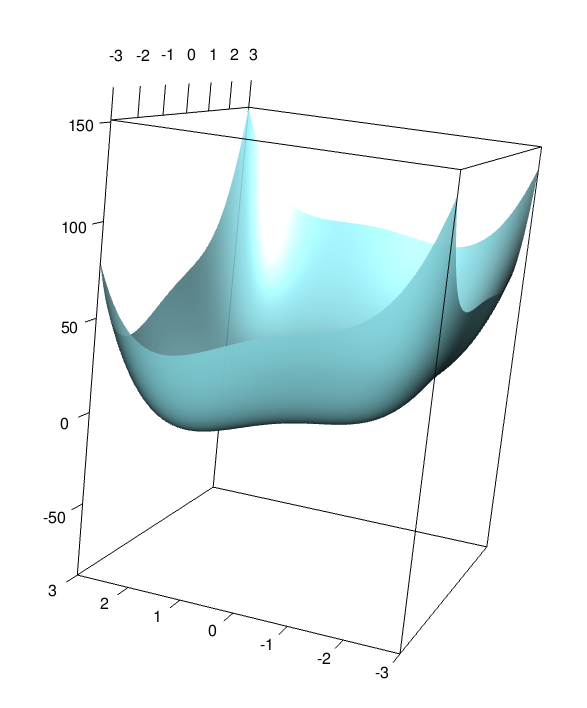
\includegraphics[width=0.7\linewidth,height=0.5\textheight]{plot-3d}

From the 3D plot, I guess the minimum point is around (-2.1, 1.8, -11).

\hypertarget{q7}{%
\subsection{Q7:}\label{q7}}

\emph{Find the partial derivatives of f with respect to x1 and x2 and
write a function called grad\_f() that gives the gradient of f.}

\textbf{MY SOLUTION:}

\begin{Shaded}
\begin{Highlighting}[]
\SpecialCharTok{\textgreater{}} \CommentTok{\# write the original function}
\ErrorTok{\textgreater{}}\NormalTok{ f\_origin }\OtherTok{\textless{}{-}} \ControlFlowTok{function}\NormalTok{(x\_1, x\_2)\{}
\SpecialCharTok{+}\NormalTok{   out\_ }\OtherTok{\textless{}{-}}\NormalTok{ x\_1}\SpecialCharTok{\^{}}\DecValTok{4}\SpecialCharTok{+}\NormalTok{x\_2}\SpecialCharTok{\^{}}\DecValTok{4{-}2}\SpecialCharTok{*}\NormalTok{x\_1}\SpecialCharTok{\^{}}\DecValTok{2}\SpecialCharTok{+}\DecValTok{2}\SpecialCharTok{*}\NormalTok{x\_1}\SpecialCharTok{*}\NormalTok{x\_2}\DecValTok{{-}3}\SpecialCharTok{*}\NormalTok{x\_2}\SpecialCharTok{\^{}}\DecValTok{2}\SpecialCharTok{+}\DecValTok{6}\SpecialCharTok{*}\NormalTok{x\_1}\DecValTok{{-}4}\SpecialCharTok{*}\NormalTok{x\_2}\SpecialCharTok{+}\DecValTok{10}
\SpecialCharTok{+}   \FunctionTok{return}\NormalTok{(out\_)}
\SpecialCharTok{+}\NormalTok{ \}}
\SpecialCharTok{\textgreater{}} 
\ErrorTok{\textgreater{}} \CommentTok{\# write the two partial derivatives}
\ErrorTok{\textgreater{}}\NormalTok{ dfdx\_1 }\OtherTok{\textless{}{-}} \ControlFlowTok{function}\NormalTok{(x\_1, x\_2)\{}
\SpecialCharTok{+}   \FunctionTok{return}\NormalTok{(}\DecValTok{4}\SpecialCharTok{*}\NormalTok{x\_1}\SpecialCharTok{\^{}}\DecValTok{3{-}4}\SpecialCharTok{*}\NormalTok{x\_1 }\SpecialCharTok{+} \DecValTok{2}\SpecialCharTok{*}\NormalTok{x\_2}\SpecialCharTok{+}\DecValTok{6}\NormalTok{)}
\SpecialCharTok{+}\NormalTok{ \}}
\SpecialCharTok{\textgreater{}}\NormalTok{ dfdx\_2 }\OtherTok{\textless{}{-}} \ControlFlowTok{function}\NormalTok{(x\_1, x\_2)\{}
\SpecialCharTok{+}   \FunctionTok{return}\NormalTok{(}\DecValTok{4}\SpecialCharTok{*}\NormalTok{x\_2}\SpecialCharTok{\^{}}\DecValTok{3}\SpecialCharTok{+}\DecValTok{2}\SpecialCharTok{*}\NormalTok{x\_1}\DecValTok{{-}6}\SpecialCharTok{*}\NormalTok{x\_2}\DecValTok{{-}4}\NormalTok{)}
\SpecialCharTok{+}\NormalTok{ \}}
\SpecialCharTok{\textgreater{}} 
\ErrorTok{\textgreater{}} \CommentTok{\# write the gradient descent function}
\ErrorTok{\textgreater{}}\NormalTok{ grad\_f }\OtherTok{\textless{}{-}} \ControlFlowTok{function}\NormalTok{(x\_1, x\_2)\{}\FunctionTok{c}\NormalTok{(}\FunctionTok{dfdx\_1}\NormalTok{(x\_1,x\_2), }\FunctionTok{dfdx\_2}\NormalTok{(x\_1,x\_2))\}}
\end{Highlighting}
\end{Shaded}

\hypertarget{q8}{%
\subsection{Q8:}\label{q8}}

\emph{Write a function to implement gradient ascent with arguments for
the start point, the number of iterations, the step size alpha\ldots{}}

\textbf{MY SOLUTION:}

\begin{Shaded}
\begin{Highlighting}[]
\SpecialCharTok{\textgreater{}}\NormalTok{ gradient\_d }\OtherTok{\textless{}{-}} \ControlFlowTok{function}\NormalTok{(f\_original, }\CommentTok{\# the original function}
\SpecialCharTok{+}\NormalTok{                        grad\_f, }\CommentTok{\# the gradient function}
\SpecialCharTok{+}\NormalTok{                        start\_point, }\CommentTok{\# the start point, a vector}
\SpecialCharTok{+}                        \AttributeTok{max\_iter=}\DecValTok{100}\NormalTok{, }\CommentTok{\# the maximum number of iteration}
\SpecialCharTok{+}                        \AttributeTok{alpha=}\FloatTok{0.03}\NormalTok{, }\CommentTok{\# learning rate/ step size}
\SpecialCharTok{+}                        \AttributeTok{epsilon=}\FloatTok{1e{-}5} \CommentTok{\# stopping criterion}
\SpecialCharTok{+}\NormalTok{ )\{}
\SpecialCharTok{+}   \CommentTok{\# initial settings}
\SpecialCharTok{+}\NormalTok{   p\_old }\OtherTok{\textless{}{-}}\NormalTok{ start\_point;i }\OtherTok{\textless{}{-}} \DecValTok{1}\NormalTok{;check }\OtherTok{\textless{}{-}} \DecValTok{1}
\SpecialCharTok{+}   \ControlFlowTok{while}\NormalTok{ (check }\SpecialCharTok{\textgreater{}}\NormalTok{ epsilon) \{}
\SpecialCharTok{+}     \CommentTok{\# print the iteration information at each 10 rounds}
\SpecialCharTok{+}     \ControlFlowTok{if}\NormalTok{ (i }\SpecialCharTok{==}\DecValTok{1} \SpecialCharTok{|}\NormalTok{ i}\SpecialCharTok{\%\%}\DecValTok{10} \SpecialCharTok{==} \DecValTok{0}\NormalTok{)\{}
\SpecialCharTok{+}      \FunctionTok{print}\NormalTok{(}\FunctionTok{paste0}\NormalTok{(}\StringTok{"Iter "}\NormalTok{, i, }\StringTok{"; f(x\_1, x\_2)= "}\NormalTok{, }\FunctionTok{f\_original}\NormalTok{(p\_old[}\DecValTok{1}\NormalTok{], p\_old[}\DecValTok{2}\NormalTok{])))}
\SpecialCharTok{+}\NormalTok{     \}}
\SpecialCharTok{+}     \CommentTok{\# Stop condition and warning}
\SpecialCharTok{+}     \ControlFlowTok{if}\NormalTok{ (i }\SpecialCharTok{\textgreater{}}\NormalTok{ max\_iter) \{}
\SpecialCharTok{+}       \FunctionTok{print}\NormalTok{(}\StringTok{"Exceed maximum number of iterations"}\NormalTok{)}
\SpecialCharTok{+}       \ControlFlowTok{break}
\SpecialCharTok{+}\NormalTok{       \}}
\SpecialCharTok{+}     \ControlFlowTok{if}\NormalTok{ (}\FunctionTok{abs}\NormalTok{(p\_old[}\DecValTok{1}\NormalTok{]) }\SpecialCharTok{\textgreater{}} \DecValTok{3} \SpecialCharTok{|}\FunctionTok{abs}\NormalTok{(p\_old[}\DecValTok{2}\NormalTok{] }\SpecialCharTok{\textgreater{}}\DecValTok{3}\NormalTok{)) \{}
\SpecialCharTok{+}       \FunctionTok{print}\NormalTok{(}\StringTok{"Exceed the Given Range"}\NormalTok{)}
\SpecialCharTok{+}       \ControlFlowTok{break}
\SpecialCharTok{+}\NormalTok{       \}}
\SpecialCharTok{+}     \CommentTok{\# load the gradient}
\SpecialCharTok{+}\NormalTok{     gradient\_ }\OtherTok{\textless{}{-}} \FunctionTok{grad\_f}\NormalTok{(p\_old[}\DecValTok{1}\NormalTok{], p\_old[}\DecValTok{2}\NormalTok{])}
\SpecialCharTok{+}     \CommentTok{\# normalize the the gradient vector}
\SpecialCharTok{+}\NormalTok{     gradient\_norm }\OtherTok{\textless{}{-}}\NormalTok{ gradient\_}\SpecialCharTok{/}\FunctionTok{sqrt}\NormalTok{(gradient\_}\SpecialCharTok{\%*\%}\NormalTok{gradient\_)}
\SpecialCharTok{+}     \CommentTok{\# update the point coordination with gradient * learning rate}
\SpecialCharTok{+}\NormalTok{     p\_new }\OtherTok{\textless{}{-}}\NormalTok{ p\_old }\SpecialCharTok{{-}}\NormalTok{ alpha}\SpecialCharTok{*}\NormalTok{gradient\_norm}
\SpecialCharTok{+}     \CommentTok{\# check the updating rate of p\_new, if less than epsilong, stop}
\SpecialCharTok{+}\NormalTok{     check }\OtherTok{\textless{}{-}} \FunctionTok{sqrt}\NormalTok{((p\_new}\SpecialCharTok{{-}}\NormalTok{p\_old)}\SpecialCharTok{\%*\%}\NormalTok{(p\_new}\SpecialCharTok{{-}}\NormalTok{p\_old))}\SpecialCharTok{/} \FunctionTok{sqrt}\NormalTok{(p\_old }\SpecialCharTok{\%*\%}\NormalTok{ p\_old)}
\SpecialCharTok{+}     \CommentTok{\# redefine the old point to send for next updating }
\SpecialCharTok{+}\NormalTok{     p\_old }\OtherTok{\textless{}{-}}\NormalTok{ p\_new}
\SpecialCharTok{+}\NormalTok{     i }\OtherTok{\textless{}{-}}\NormalTok{ i }\SpecialCharTok{+} \DecValTok{1}
\SpecialCharTok{+}\NormalTok{   \}}
\SpecialCharTok{+}   \FunctionTok{print}\NormalTok{(}\FunctionTok{paste0}\NormalTok{(}\StringTok{"The minimum point is around "}\NormalTok{, }
\SpecialCharTok{+}                \FunctionTok{round}\NormalTok{(p\_old[}\DecValTok{1}\NormalTok{],}\DecValTok{4}\NormalTok{),}\StringTok{" "}\NormalTok{,}
\SpecialCharTok{+}                \FunctionTok{round}\NormalTok{(p\_old[}\DecValTok{2}\NormalTok{],}\DecValTok{4}\NormalTok{),}\StringTok{" "}\NormalTok{,}
\SpecialCharTok{+}                \FunctionTok{round}\NormalTok{(}\FunctionTok{f\_origin}\NormalTok{(p\_old[}\DecValTok{1}\NormalTok{],p\_old[}\DecValTok{2}\NormalTok{]),}\DecValTok{4}\NormalTok{)))}
\SpecialCharTok{+}\NormalTok{ \}}
\end{Highlighting}
\end{Shaded}

Then, try this gradient descent method on the given function.

\begin{Shaded}
\begin{Highlighting}[]
\SpecialCharTok{\textgreater{}} \FunctionTok{gradient\_d}\NormalTok{(f\_origin, grad\_f, }\FunctionTok{c}\NormalTok{(}\DecValTok{1}\NormalTok{,}\DecValTok{2}\NormalTok{))}
\NormalTok{[}\DecValTok{1}\NormalTok{] }\StringTok{"Iter 1; f(x\_1, x\_2)= 15"}
\NormalTok{[}\DecValTok{1}\NormalTok{] }\StringTok{"Iter 10; f(x\_1, x\_2)= 10.5754827068404"}
\NormalTok{[}\DecValTok{1}\NormalTok{] }\StringTok{"Iter 20; f(x\_1, x\_2)= 7.48319133042501"}
\NormalTok{[}\DecValTok{1}\NormalTok{] }\StringTok{"Iter 30; f(x\_1, x\_2)= 5.07775708084357"}
\NormalTok{[}\DecValTok{1}\NormalTok{] }\StringTok{"Iter 40; f(x\_1, x\_2)= 2.58313967447279"}
\NormalTok{[}\DecValTok{1}\NormalTok{] }\StringTok{"Iter 50; f(x\_1, x\_2)= {-}0.242482652266101"}
\NormalTok{[}\DecValTok{1}\NormalTok{] }\StringTok{"Iter 60; f(x\_1, x\_2)= {-}3.34386884955452"}
\NormalTok{[}\DecValTok{1}\NormalTok{] }\StringTok{"Iter 70; f(x\_1, x\_2)= {-}6.45537944677232"}
\NormalTok{[}\DecValTok{1}\NormalTok{] }\StringTok{"Iter 80; f(x\_1, x\_2)= {-}9.11743349118743"}
\NormalTok{[}\DecValTok{1}\NormalTok{] }\StringTok{"Iter 90; f(x\_1, x\_2)= {-}10.6832761634467"}
\NormalTok{[}\DecValTok{1}\NormalTok{] }\StringTok{"Iter 100; f(x\_1, x\_2)= {-}10.8258617496505"}
\NormalTok{[}\DecValTok{1}\NormalTok{] }\StringTok{"Exceed maximum number of iterations"}
\NormalTok{[}\DecValTok{1}\NormalTok{] }\StringTok{"The minimum point is around {-}1.5549 1.6273 {-}10.8211"}
\end{Highlighting}
\end{Shaded}

For text space concern, I choose to print the iteration information at
each 10 rounds.The final result shows that the minimum point is around
(-1.5549, 1.6273, -10.8211), which is close to the observed possible
minimum point (-2.1, 1.8, -11) (in my response to Question 6).

\hypertarget{q9}{%
\subsection{Q9:}\label{q9}}

\emph{Write a function to implement gradient ascent with arguments for
the start point, the number of iterations, the step size alpha\ldots{}}

\textbf{MY SOLUTION:}\\
If one wants to make the steepest descent, they can adjust the learning
rate(step size). But one caveat is, a big step size will cause the point
oscillating around the minimum point and possible never reaching the
target. So, a dynamic learning rate is necessary, That is, the learning
rate can adaptively change itself from big size at the beginning to
small when closing to the target.

\end{document}
